\section*{Overview}

Li Chao tree is the structure I use when the convex hull trick is conceptually right but the nice monotone assumptions
are gone. It stores a dynamic set of lines and answers ``which line is best at \(x\)?'' queries in logarithmic time on
a fixed coordinate domain.

\section*{When to Use It}

Use a Li Chao tree when:

\begin{itemize}
  \item the recurrence or query is of the form \(\min (mx + b)\) or \(\max (mx + b)\),
  \item line insertion order is arbitrary,
  \item query \(x\)-values are arbitrary,
  \item the coordinate domain can be bounded in advance or compressed offline.
\end{itemize}

It is the standard fallback when the monotone deque version of the convex hull trick is not legal.

\section*{Core Idea}

Each node of the segment tree owns an interval of \(x\)-values and stores one candidate line. When a new line is
inserted, compare it with the stored line at the midpoint:

\begin{itemize}
  \item the better line at the midpoint stays in the current node,
  \item the worse line is pushed into the half-interval where it might still win.
\end{itemize}

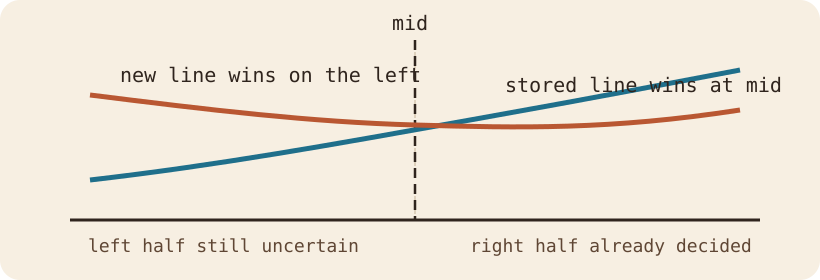
\includegraphics[width=\textwidth]{figures/query-partition.svg}

\section*{Key Insight}

Two lines intersect at most once. That means if one line is better than another at the midpoint, the only place where
the other line can still matter is on one side of that midpoint. The insert step exploits exactly that one-crossing
property.

\section*{Operations / Main Technique}

\begin{itemize}
  \item insert one line,
  \item query the minimum or maximum value at one \(x\),
  \item optionally compress \(x\)-coordinates first if only a known query set matters.
\end{itemize}

\paragraph{Worked example.}
Suppose a node covers \([0, 8]\) with midpoint \(4\). If the existing line is better at \(4\) but the new line is
better at \(8\), the new line only needs to recurse into the right half. The left half is already safe.

\section*{Correctness Intuition}

For every \(x\), at least one line on the root-to-leaf path is optimal at that \(x\). Insertions preserve that
invariant because the current node always keeps a line that wins at the midpoint, and the losing line is only sent into
the side where an intersection could still make it relevant.

\section*{Complexity Analysis}

If the domain spans \(X\) discrete coordinates:
\begin{itemize}
  \item insert: \(O(\log X)\),
  \item point query: \(O(\log X)\),
  \item memory: \(O(\text{number of inserted lines} \cdot \log X)\) for the dynamic-node version.
\end{itemize}

\section*{Implementation}

The code uses a dynamic-node minimum Li Chao tree on integer \(x\)-coordinates. That keeps the memory proportional to
the parts of the domain that are actually touched.

\section*{Common Pitfalls}

\begin{itemize}
  \item Using Li Chao when the functions are not lines or do not have the one-intersection property.
  \item Picking a domain that does not actually cover all queried \(x\)-values.
  \item Forgetting that the structure answers point queries, not arbitrary interval minima by itself.
  \item Overflow in \(mx + b\) when both \(m\) and \(x\) are large.
\end{itemize}

\section*{Variants / Extensions}

\begin{itemize}
  \item Maximum queries instead of minimum queries.
  \item Li Chao segment tree with lines active only on subsegments.
  \item Offline compressed-domain Li Chao when only specific query coordinates matter.
\end{itemize}

\section*{Practice Problems}

\begin{itemize}
  \item DP recurrences with arbitrary line insertion order.
  \item Maintain a dynamic lower envelope of linear costs.
  \item Segment-restricted line insertion after offline event expansion.
\end{itemize}

\section*{References}

\begin{itemize}
  \item \href{https://cp-algorithms.com/geometry/convex_hull_trick.html}{cp-algorithms: Convex Hull Trick and Li Chao Tree}.
  \item \href{https://codeforces.com/catalog?locale=en}{Codeforces Catalog}.
  \item \href{https://github.com/kth-competitive-programming/kactl}{KACTL}.
\end{itemize}
